\documentclass{article}
\usepackage[utf8]{inputenc}
\usepackage[a4paper]{geometry}
\usepackage{graphicx}
\usepackage{amsmath}
\usepackage{mathtools}
\usepackage{biblatex} 
\addbibresource{references.bib}

\title{Velocity drift correction using ordinary least squares for displacement measurement with a MPU-6050 sensor}
\author{Quazi Irfan, Marco Ciarcià, Gary Hatfield}

\begin{document}

\maketitle
\begin{abstract}

This paper introduces an algorithm to improve displacement estimation from accelerometer measurements captured by an inertial measurement sensor. Noise is an inherent characteristics of micro electro-mechanical system based inertial sensors, and these noises show up as drift when integrating the acceleration signal to obtain velocity and integrating velocity signal to obtain displacement. The proposed algorithm estimates the drift in velocity signal by fitting a straight line. The estimated drift is then subtracted from the velocity signal. Displacement calculated from this updated velocity signal are much improved and it is very close to the true displacement, which was captured by an external high precision camera.

\end{abstract}
\section{Introduction}
Inertial measurement unit(IMU) measures linear acceleration, angular velocity and magnetic heading using accelerometer, gyroscope and magnetometers. Nowadays, Micro Electro-Mechanical System (MEMS) based IMU sensors have become ubiquitous features is everyday electronics. One of its many usages of this sensor is inertial navigational system. It may appear that a sensor measuring acceleration could easily measure displacement by integrating the acceleration twice - but this process suffers from accumulation error(specifically for MEMS based sensors). As the accelerometer data is being integrated twice to calculate velocity and displacement, any small measurement error will accumulate over time. This leads to drift in velocity and subsequently larger drift in displacement \cite{woodman2007introduction}. This drift can be removed in a few different ways \cite{han_random_2020}. One approach is to fusing inertial sensors with another sensor that does not drift. Notable example is the inertial navigational system used by Mars 2020 Helicopter built by NASA. This system is fusing camera vision and IMU sensors using extended Kalman filter \cite{bayard_vision-based_2019}. The drift can also be removed by filtering the signal at different stages. One study have used Kalman filter to smooth accelerometer signal before integrating it twice\cite{pang_evaluation_nodate}. A recent study proposed a heuristics to remove drift from velocity signal by testing if the rate of change in velocity is too small \cite{du2015signal}. Some studies have  calculated displacement from accelerometer by taking the Fourier transform of the accelerometer signal, followed by division by the angular frequency and taking an inverse Fourier transformation of the resultant signal. But this approach produces no less noisy displacement than integrating the acceleration signal twice \cite{brandt2014integrating, han2003retrieving}.

This aim of this paper is to provide a method to estimate and remove drift in the velocity signal by fitting a straight using ordinary least squares which improves the accuracy of calculated displacement.

\section{Methodology}
In this study, the sensor is kept stationary at startup for a few seconds to collect and average the first 1000 samples to calculate the turn-on bias of the accelerometer. This bias is then subtracted from any subsequent measurements. This study processes the accelerometer data offline - therefore the accelerometer data is collected and saved to a file. The offline processing step starts by applying a threshold $0.03g$(obtained experimentally) to the accelerometer data. Then the accelerometer data is multiplied by 9.81 to convert the unit to $ms^{-2}$, which is followed by an optional 12 sample rolling average. Trapezoidal numerical integration method is used to find velocity from this accelerometer data. 

The velocity data can be numerically integrated once again to find the displacement. But as accelerometer in-run bias drift\footnote{The output value of the accelerometer sensor do not return to zero when it comes to rest after motion. This is called in-run bias or bias instability. This bias can be positive or negative.} causes drift in velocity. Integrating velocity data with drift produces inaccurate displacement. In this study drift will be removed from the velocity signal. To remove the drift a linear function is fit to the velocity signal using ordinary least squares. The fitted line is then subtracted from the velocity data to remove linear drift. To remove drift even further another $0.25\ ms^{-1}$(obtained experimentally) threshold is applied. Trapezoidal numerical integration method is then applied on the resultant drift free velocity signal to obtain the displacement. Displacement obtained through this process is then compared with displacement measured by an external high precision camera(OptiTrack Prime 13 camera), to validate the accuracy. This high precision camera is a room sized multi camera setup that can track special markers attached to a moving body within sub-millimeter accuracy.

\begin{figure}[htp]
    \centering
    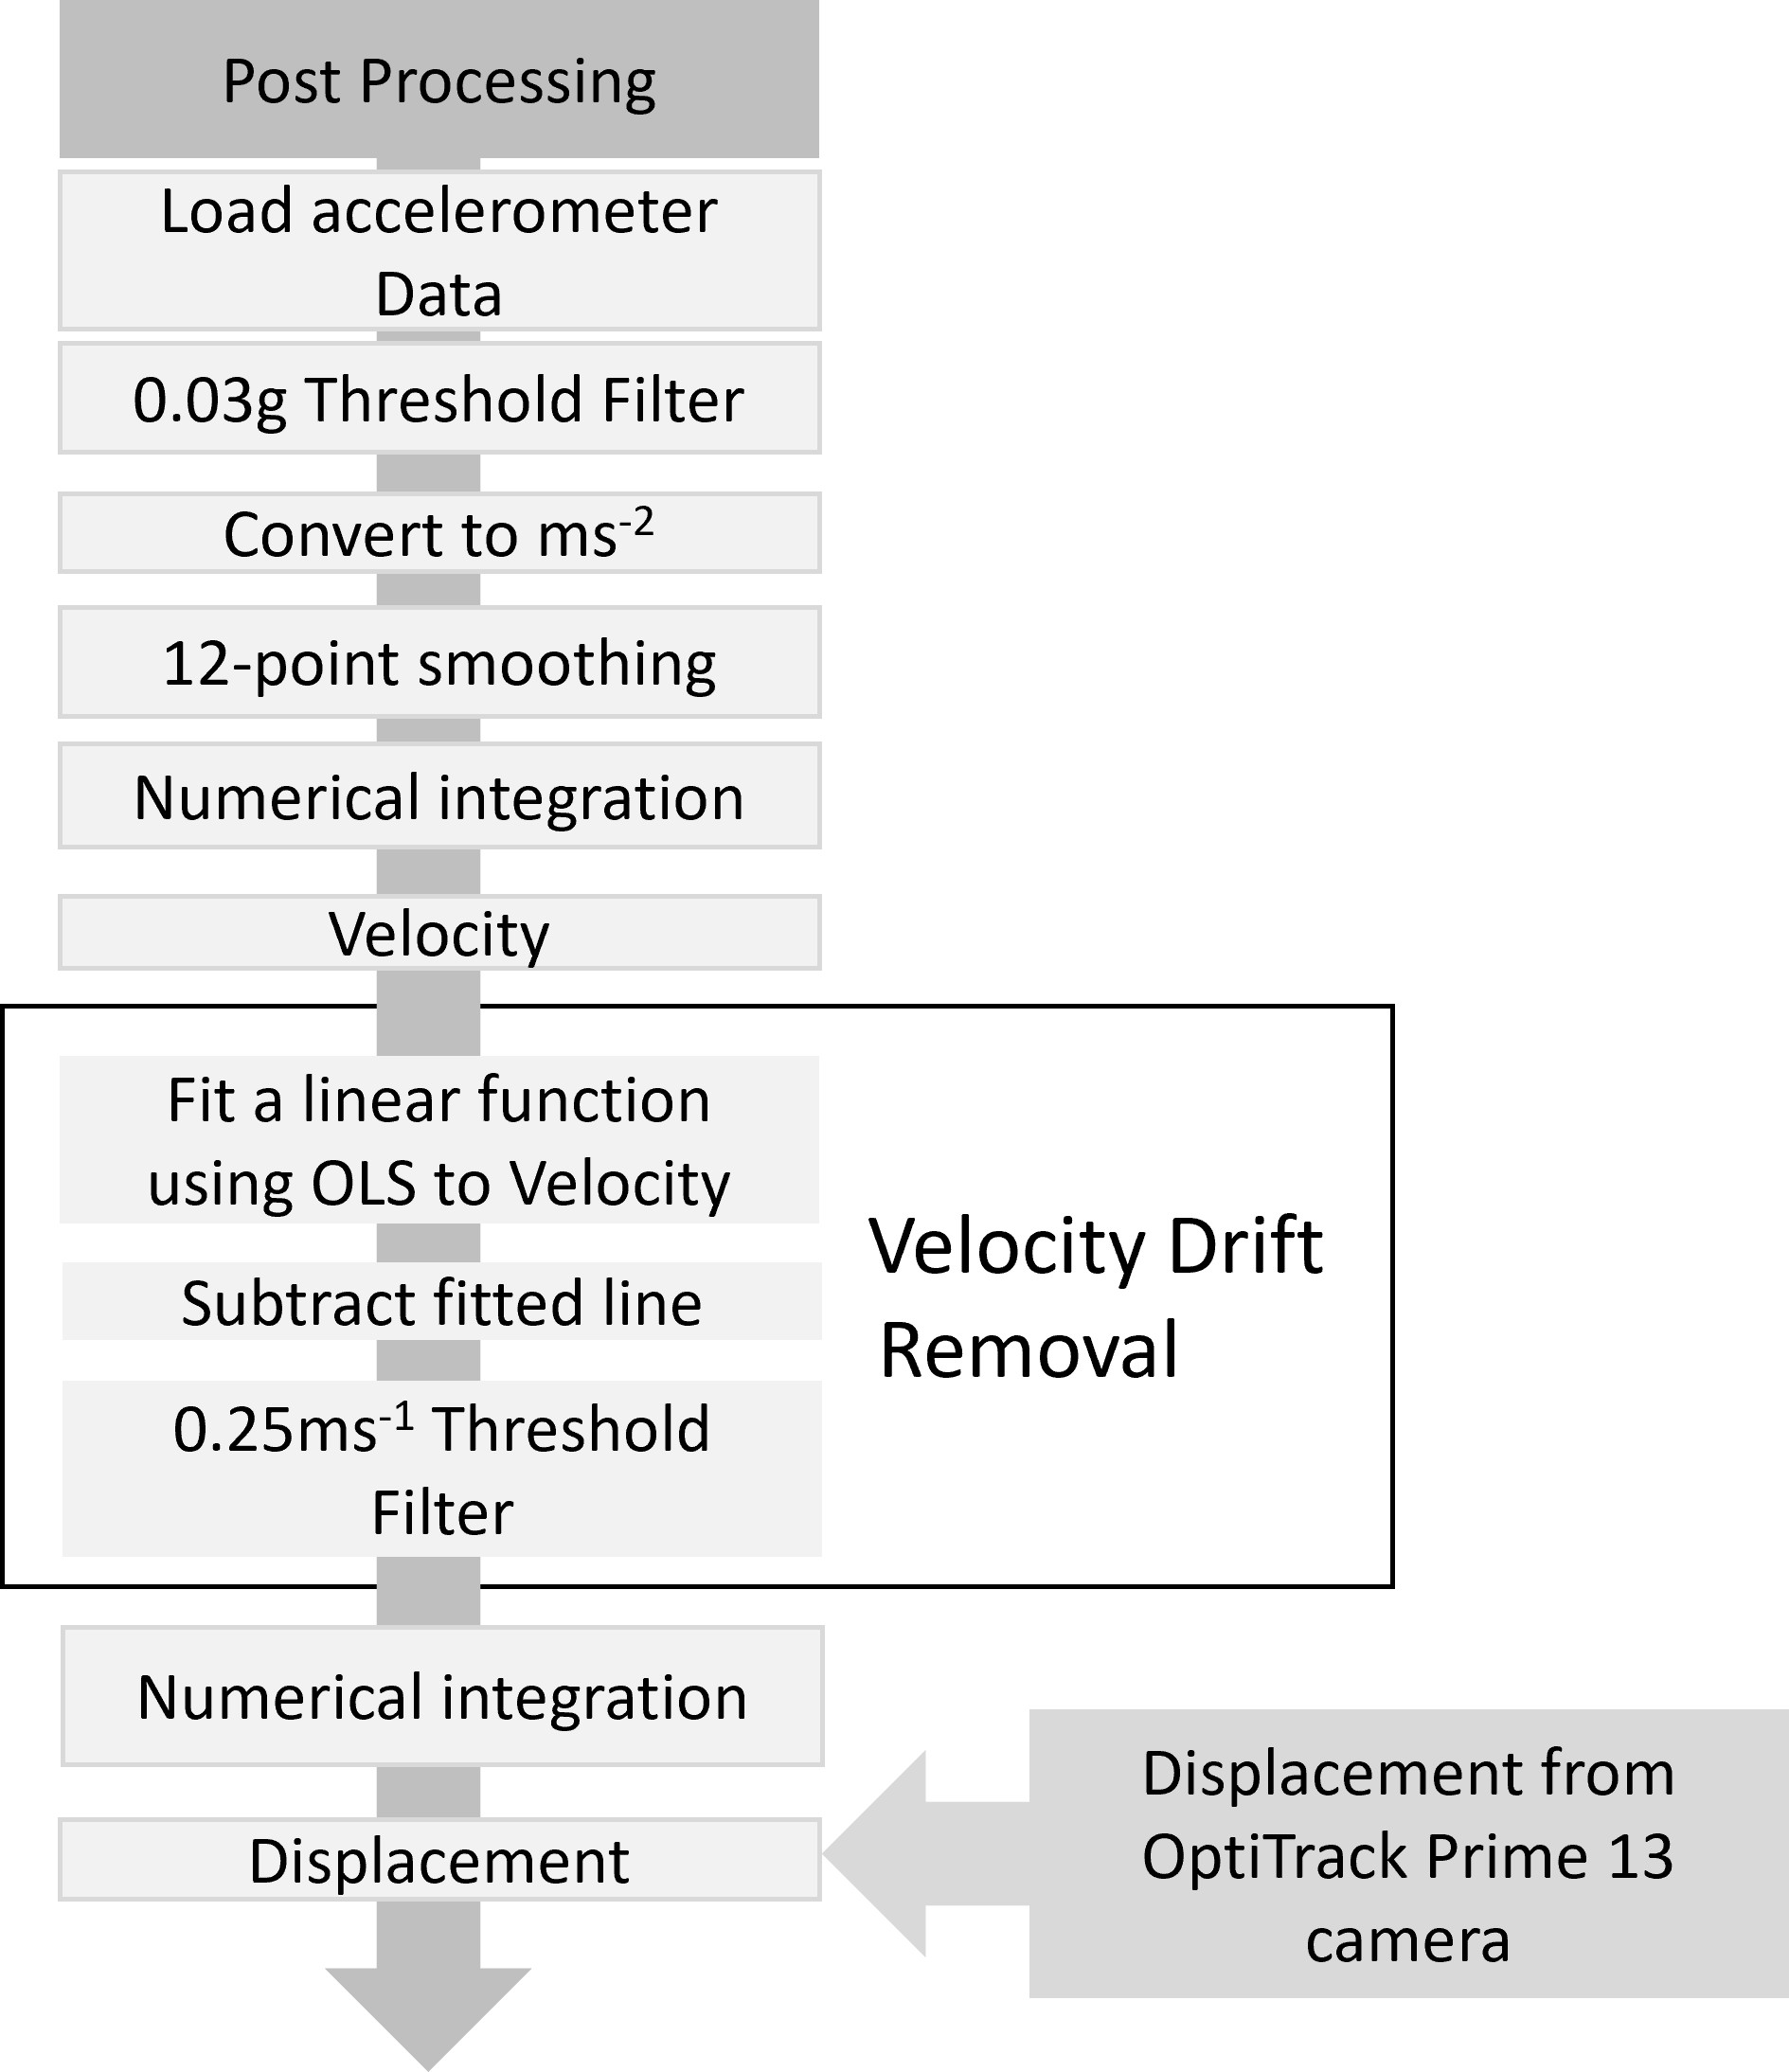
\includegraphics[width=8cm]{1.png}
    \caption{Flowchart of sensor recording and velocity drift removal}
\end{figure}

\subsection{Displacement from Acceleration}
An accelerometer measures linear acceleration. Linear displacement can be obtained by integrating linear acceleration twice. If $a$, $v$ and $s$ represent the acceleration, velocity and displacement signal respectively then,

$$v = \int a \,dt$$

$$s = \int v \,dt$$

Closed form of accelerometer data is not available. But acceleration values at discrete time stamps are available, and therefore a numerical integration method will be used to obtain velocity from acceleration and displacement from velocity.

\subsection{Numerical Integration}
The Trapezoidal method will be used to perform numerical integration. It is an improvement over rectangular numerical integration method. Rectangular method can be used when the recording session is small, and sampling rate of the sensor is high. Since some of our recordings are about 60 seconds long, using the Trapezoidal method improved accuracy of integration. Using this method, value of velocity at time $i$ is the following \cite{seifert2007implementing},
$$v_i = v_{i-1} + a_i \Delta t + \frac{1}{2}|a_i - a_{i-1}| \Delta t$$

Similarly, value of displacement at time $i$ can be obtained by the following,
$$s_i = s_{i-1} + v_i \Delta t + \frac{1}{2}|v_i - v_{i-1}| \Delta t$$

Here $\Delta t$ is the sampling frequency and $i$ is the time index that goes from $0$ to $n$.

\subsection{Threshold and Smoothing Filter}
The accelerometer does not always output zero when stationary even after removing turn-on bias. To fix this problem a threshold filter needs to be applied to the accelerometer data. In this filter, accelerometer value is set to zero if its absolute value is smaller then the threshold value. If $x_i$ is the input accelerometer signal at time $i$ after applying threshold at $\delta$ the output signal is $t_i$ using the following,

\begin{equation}
  t_i =
    \begin{cases}
      0 & \text{; if }|x_i| \le \delta \nonumber \\
      x_i & \text{; otherwise} 
    \end{cases}       
\end{equation}

A rolling average is used as a smoothing/low pass filter for this study. This kind of filter is optimal to reduce random noise while retaining sharp edges. Moving average filter is a good filter for signal that contains information in time domain and accelerometer encodes data in time domain\cite{smith2013digital}. If $x_i$ is the input signal, after applying $l$ point rolling average, the output smoothed signal will be $s_j$, where $j$ ranges from $l$ to $n$,

$$s_j = \frac{1}{l} \sum_{i=1}^l x_{j-i}$$

This illustrates that the smoothed signal is smaller($j < i$) than the input signal. Therefore it was padded with zeroes to simplify plotting. In this study, estimated displacement did not improve significantly with or without this filter.

\subsection{Fitting a straight line using ordinary least square(OLS) method}
A straight line was constructed that best fit the velocity graph. There are multiple ways to fit a straight line through some data points. Ordinary least squares is one of those methods where the objective function is to minimize the sum of squared difference of the data points and the straight line. This straight line can be seen as the green line in Fig 3.

Here is the model to fit a straight line through some velocity data $v_i$. $\beta_0$ and $\beta_1$ are the intercept and slope of the straight line respectively. $\epsilon$ is the residual, which is the vertical distance between the velocity data and straight line at a given time index $i$.
$$V_i = \beta_0 + \beta_1 v_i + \epsilon_i$$

OLS method provides an estimation for the intercept $\beta_0$ and slope $\beta_1$. The objective function for this model is to find the value of $\beta_0$ and $\beta_1$ the minimized the sum of squared residual. The object function is the following,
\begin{equation}
\min_{\beta_0\ \beta_1} \sum \epsilon_i^2 = \min_{\beta_0\beta_1}  \sum_{i=1}^{n}(V_i - \hat{\beta_0} - \hat{\beta_1}v_i)^2 \nonumber
\end{equation}

OLS estimators for intercept $\beta_0$ and slope $\beta_1$ are the following,\footnote{Derivation of $\beta_0$ and $\beta_1$ are in the appendix.}
$$\hat{\beta_1} = \frac{n\bar{v}\bar{V} - \sum_{i=1}^{n} v_iV_i}{\sum_{i=1}^{n} v_i^2 - n\bar{v}^2}$$

$$\hat{\beta_0} =  \bar{V} - \hat{\beta_1}\bar{v}$$

Note that both $\beta_0$ and $\beta_1$ can be calculated as new sample arrives. Time complexity\footnote{Time complexity is the computational complexity that describes the amount of computer time it takes to run an algorithm.} to calculate $\beta_0$ and $\beta_1$ is constant or $O(n)$ which allows them to run in real time as $n$ is the number of new samples, usually one, that is affecting the best fit straight line.

\section{Experimental Setup}
In this study, MPU-6050 IMU breakout board and a Arduino Uno was be mounted on a full size breadboard. Arduino Uno was connected to a laptop via an USB cable. A Python script running on the laptop was recording accelerometer sensor and saving to a file for post processing. Sensor data was recorded for a prespecified period of time. In each recording session, the sensor was turned on and kept stationary while it calculates the turn-on bias. After that the sensor was moved by hand, and the Python script would record and save the accelerometer data that was stream to the laptop in via serial port. Each session was saved in a comma separated file(CSV) file with time stamp with for post processing.

Total 8 sessions were recorded. Session length varied from 10 to 60 seconds. For each session, sensor was moved along y axis for 30 centimeter, and after a brief pause brought back to the starting position. This periodic movement was repeated as many time possible. 

\subsection{Hardware Setup}
MPU-6050 sensors were chosen for this study as its breakout board produced by HiLetgo is inexpensive\footnote{Three breakout boards cost \$10.0}. This sensor can detect linear acceleration from $\pm$2g to $\pm$16g range which is sufficient for this study. The gyroscope can measure angular velocity from $\pm$250$^{\circ}$/sec to $\pm$2000 $^{\circ}$/sec range. This sensor also contains a temperature sensor that can be used to calibrate the sensitivity scale factor. Accelerometer can be sampled at 1kHz and the gyroscope can be sampled at 8kHz.

MPU-6050 breakout board was connected to Arduino Uno through $\text{I}^2\text{C}$(Inter-Integrated Circuit) interface. Arduino Uno was connected to a laptop using UART(Universal asynchronous receiver-transmitter) interface. The setup to connect single MPU-6050 to an Arduino Uno can be found in the following figure,
\begin{figure}[htp]
    \centering
    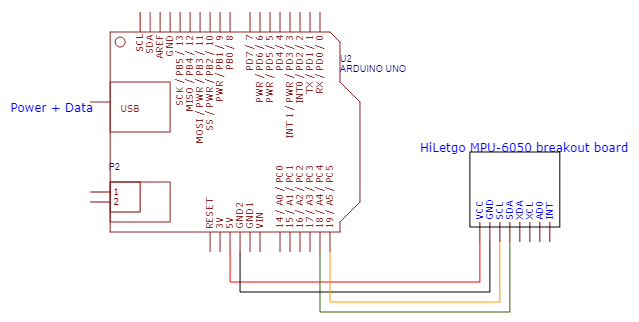
\includegraphics[width=8cm]{uno_mpu.png}
    \caption{Arduino Uno and HiLetgo MPU-6050 Breakout board connected over $\text{I}^2\text{C}$ }
\end{figure}

\subsection{Software Setup}
\subsubsection{Arduino Firmware}
Reading and writing data to MPU-6050 is done via reading and writing to registers. For example, to be set the sensitivity of MPU-6050 to $\pm$2g, bit 3 and 4 of 28th or 0x1c register needs to set to 00. Accelerometer output is placed in 59th to 64th register. Each axis of the accelerometer output is a signed 16 bit integer. For example, registers 61 and 62 contain the  accelerometer measurement along the y-axis. In Arduino Uno, the code reads the data as fast as possible and sends the data to the connected laptop over UART connection set to 9600 Baud rate. 

MPU-6050 maps the accelerometer measurements to discrete values using signed 16 bit analog to digital converter(ADC). Before converting analog data to discrete values an analog anti-aliasing filter is used to remove any frequencies above Nyquist frequency. This is followed by another digital low pass filter(DPLF), built into MPU-6050, that can be tuned by setting appropriate value to the 26th register. In this study, the cut off frequency is set to 5Hz. This particular cut off value adds 19 milliseconds delay to the output. The 16 bit signed ADC ranges from -32,768 to 32,767, and for this sensitivity the ADC output needs to be divided by the 16384 sensitivity scale factor to convert the output value to $g$\footnote{1g = 9.81 $ms^{-2}$}. Although Accelerometer can be sampled at 1kHz, the built in digital low pass filter, $\text{I}^2\text{C}$ bus to send the data to Arduino Uno, and UART bus that send the data to laptop constrains sampling rate \cite{invensense}.

\subsubsection{Desktop Software}
Python script running on the laptop saves the stream of accelerometer values in a CSV file for post processing. The first step of post processing is to apply a threshold filter at 0.03g to remove unwanted accelerometer noise. This is implemented as a Python function that takes the signal and a threshold value and returns the modified signal. Next step is to multiplying the accelerometer values with 9.81 which is implemented using Python's list comprehension feature. The smoothing filter is also implemented as a Python function that takes in the signal the length of the filter. Trapezoid numerical integration is implemented as another Python function that takes a signal and the sampling frequency of the signal and return the integrated signal. Fitting a straight line through the velocity data is accomplished using the polyfit function from Numpy Python library. Finally, all plotting of these signals was done using Matplotlib library. 

\section{Result}
Five recorded sessions, figure 3 to 7, are plotted in this section. For each session 6 plots are generated. Fig 3 is a 10 second long recorded session. In this session the sensor was moved 30 cm along the y axis and brought back to its starting position once. Fig 3(i) is the graph of acceleration value after applying the threshold filter(0.03g), converting to in $ms^{-2}$ and smoothing filter of length 12. Fig 3(ii) is the velocity graph obtained by applying Trapezoidal numerical integration to acceleration signal. Fig 3(iii) is the displacement graph obtained by applying Trapezoidal method to the velocity signal from Fig 3(ii). The displacement graph says the sensor was moved 2 meters from its original position when the true displacement is zero.

A straight line will be fit to the velocity signal to estimate and remove the drift. In figure 3(iv), the best fit line(green line) is subtracted from the velocity data(blue line) resulting in the velocity signal without drift (orange curve). Another threshold filter is applied to remove further residual drift. In fig 3(v)  the blue curve original velocity curve and the orange curve is the new velocity signal after applying threshold.

In Fig 3(vi), the blue line is the result of Trapezoidal numerical integration applied to the drift removed velocity curve. In the same figure, the dotted orange line shows the true displacement measured from the external high precision external camera. As it can be seen these curves are very close to each other even after 60 seconds later. The 2 meter drift has mostly disappeared. Similarly, Fig 4-7 are plots from another sessions of length 20 and 60 seconds. As it can be seen from 3(vi), 4(vi), 5(vi), 6(vi) and 7(vi) that displacement calculated by the inertial sensor is very close to the true displacement measured by the external camera. Note that there is an offset in two displacement signal that is growing with time and this will be investigated in a future study.

\begin{figure}[hbt!]
  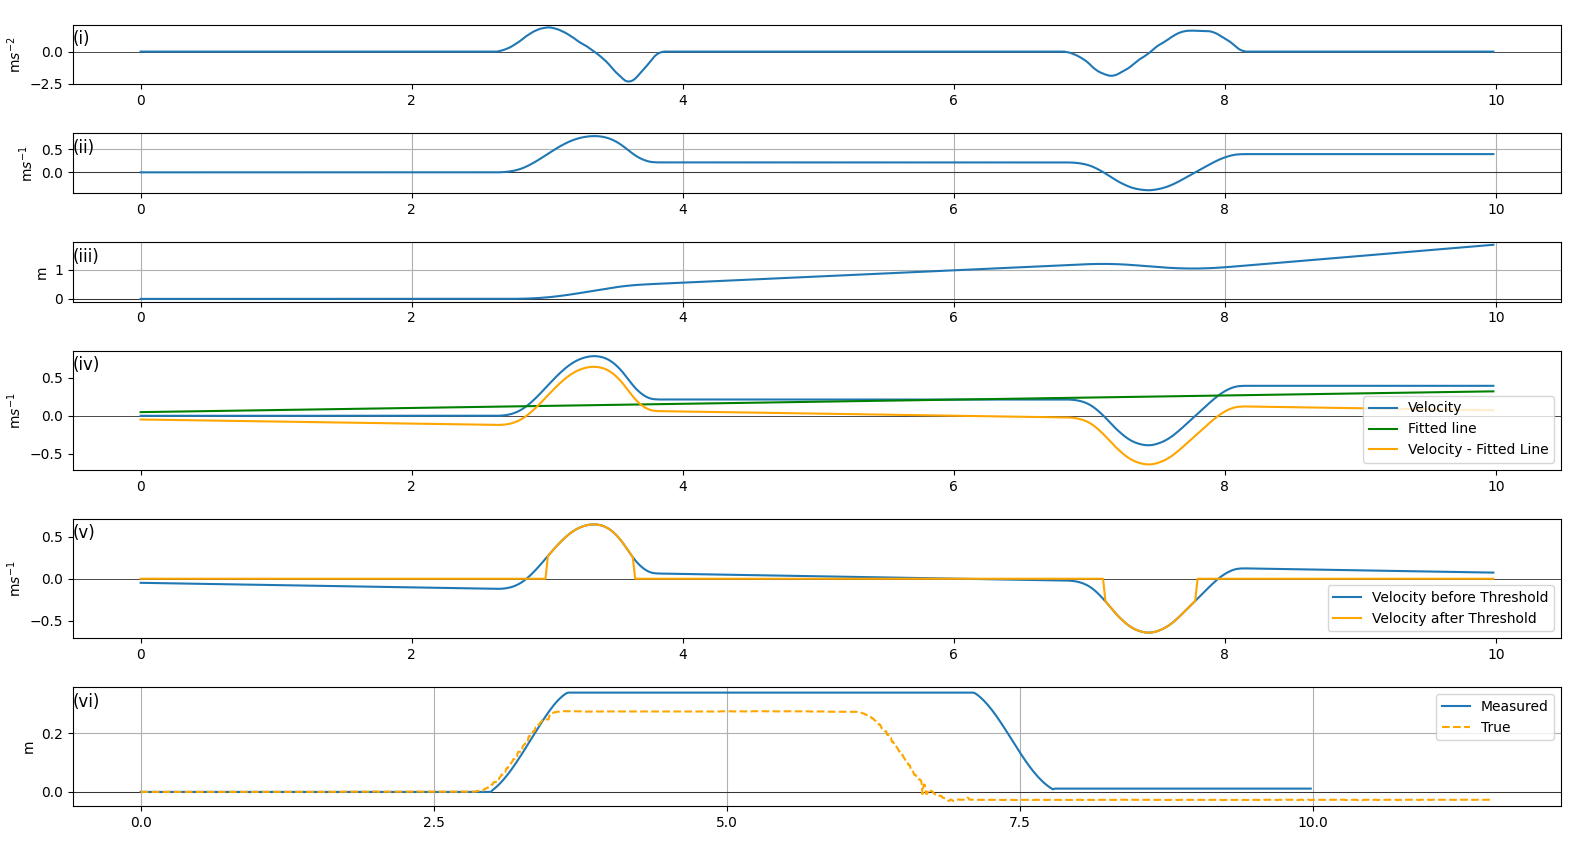
\includegraphics[width=\textwidth]{10.png}
  \caption{Moving sensor once in 10 seconds}
\end{figure}

\begin{figure}[hbt!]
  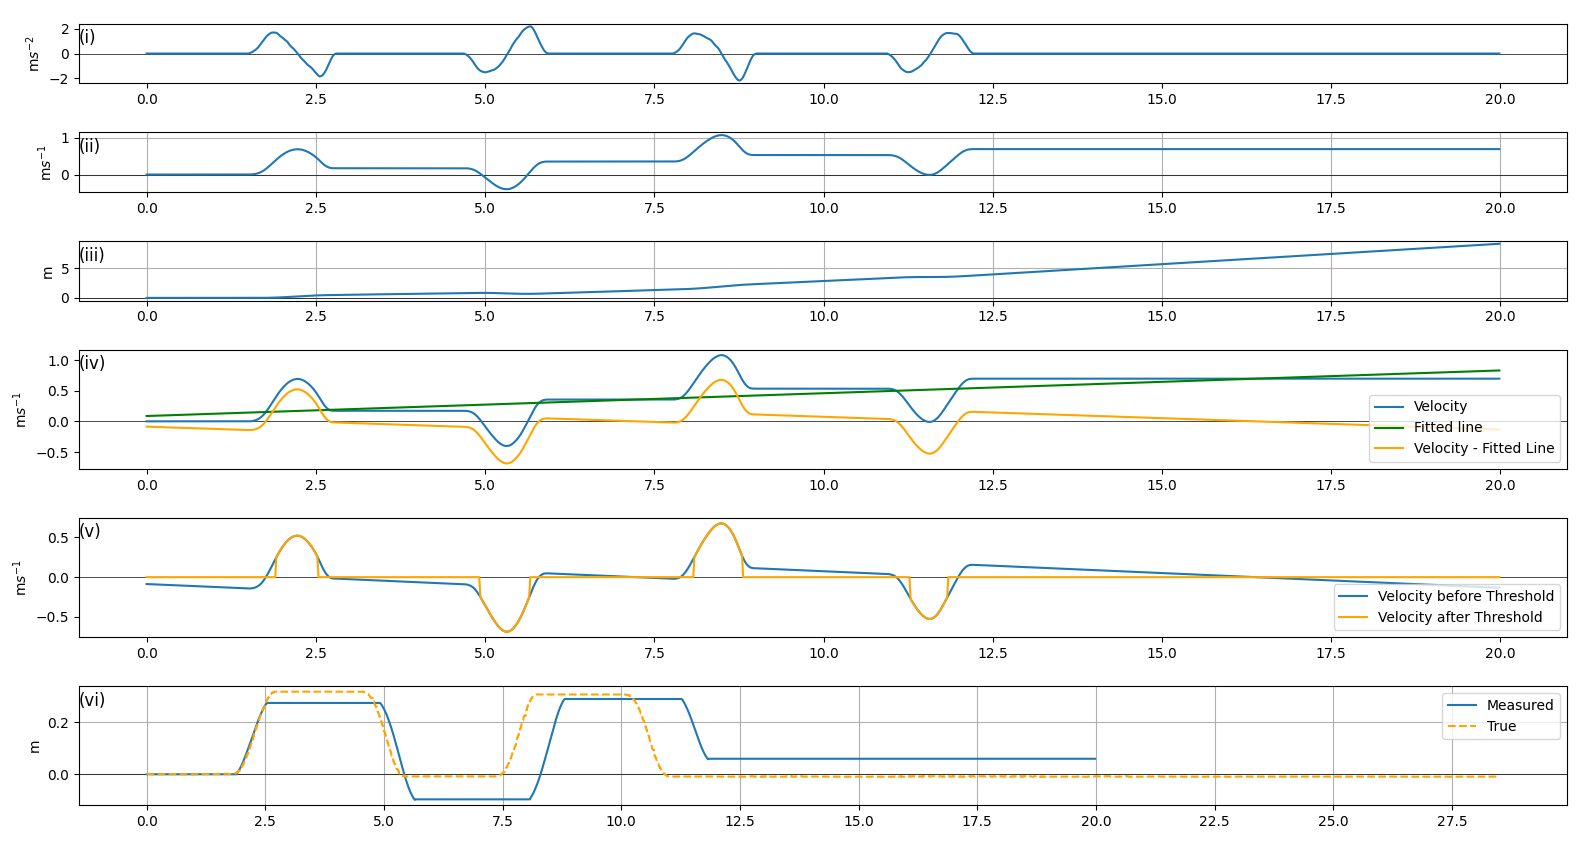
\includegraphics[width=\textwidth]{11.png}
  \caption{Moving sensor twice in 20 second}
\end{figure}

\begin{figure}[hbt!]
  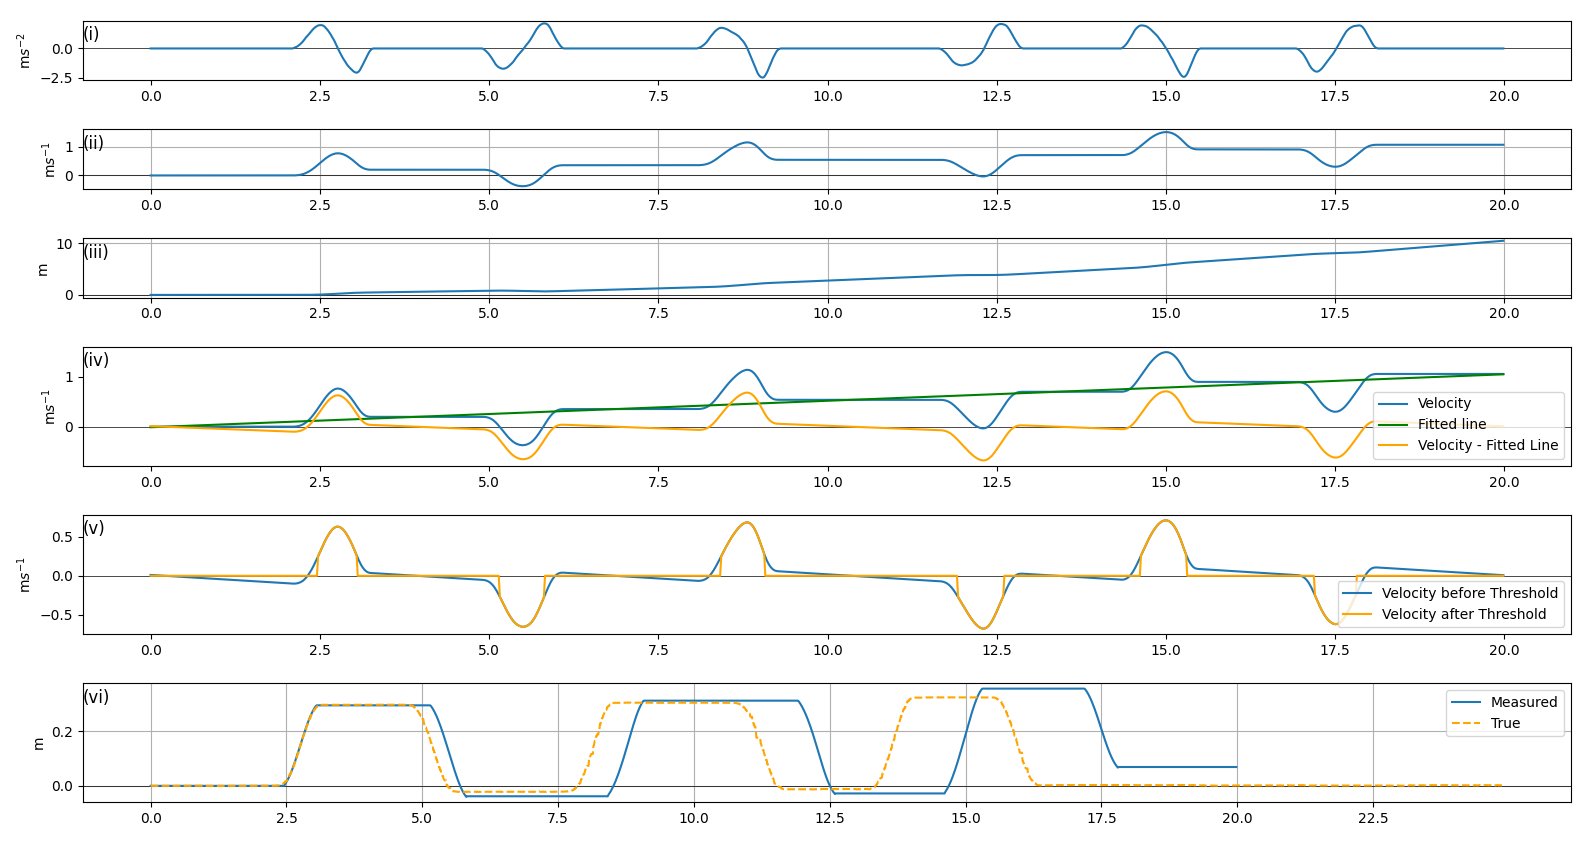
\includegraphics[width=\textwidth]{12.png}
  \caption{Moving sensor three times in 20 second}
\end{figure}

\begin{figure}[hbt!]
  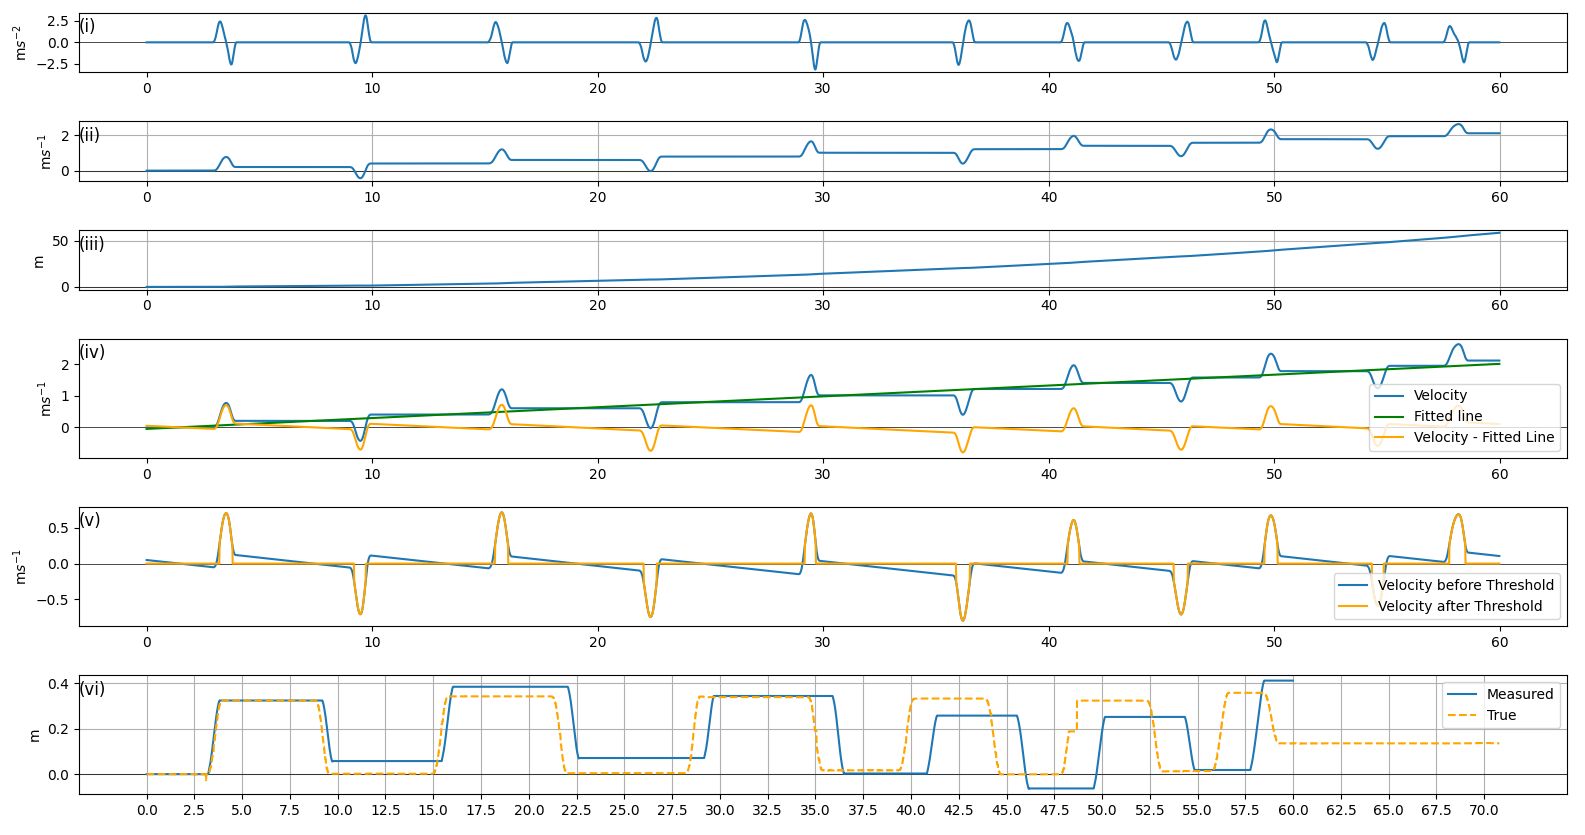
\includegraphics[width=\textwidth]{16.png}
  \caption{Moving sensor about six times in 60 second}
\end{figure}

\begin{figure}[hbt!]
  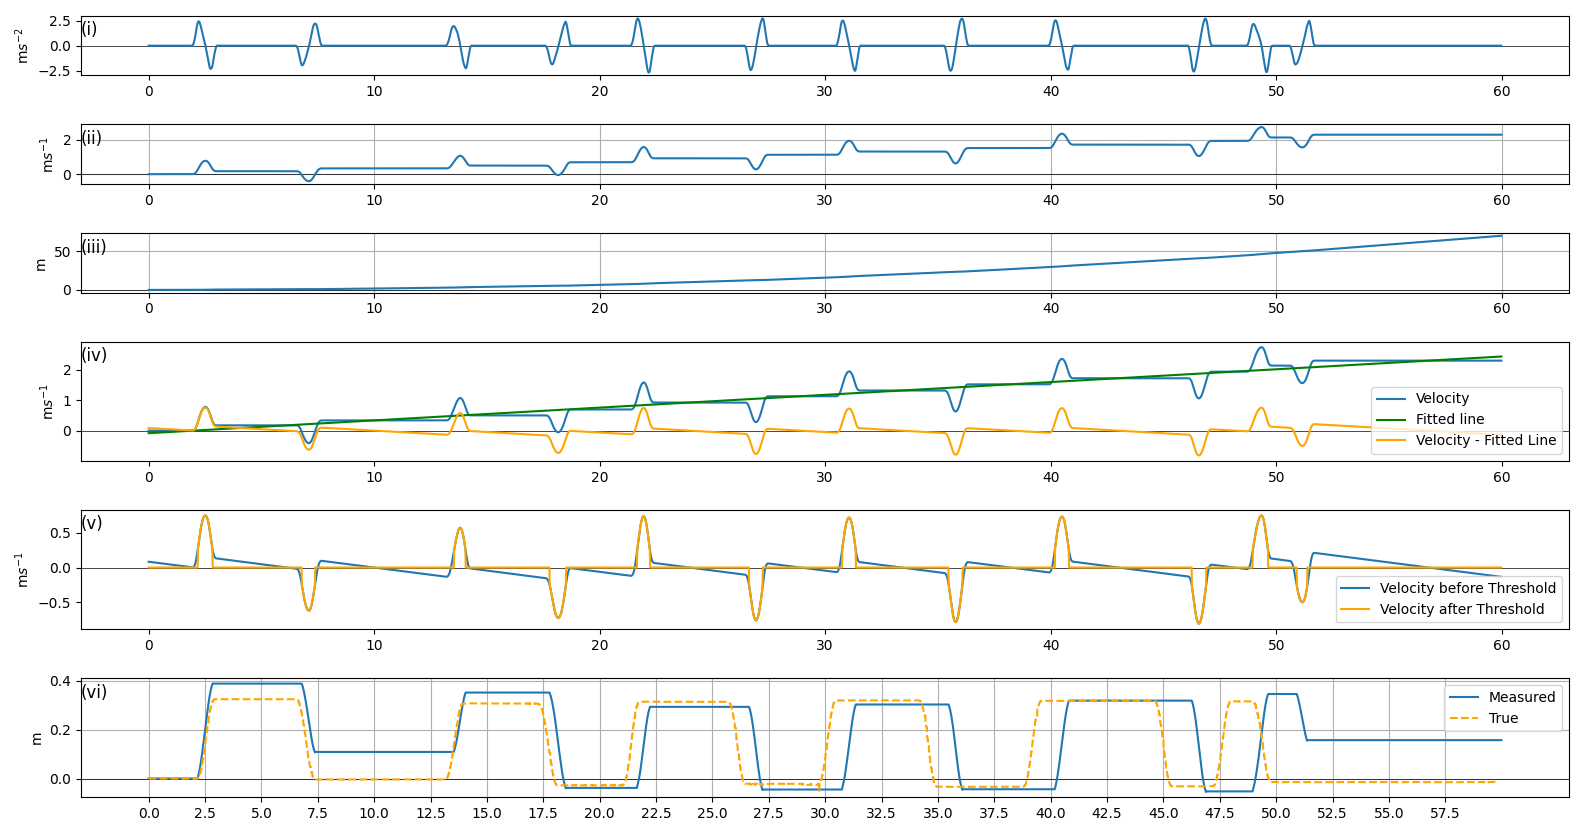
\includegraphics[width=\textwidth]{17.png}
  \caption{Moving six times in 60 second}
\end{figure}

\pagebreak

\section{Conclusion}
Calculating displacement from accelerometer can be difficult due to to error accumulation in the numerical integration. This study provides an algorithm to reduce drift in the velocity signal that improves the displacement calculation. It has identified that the accumulation error, due to integrating the acceleration signal, shows up as a linear drift in the velocity signal. This linear drift can be removed by subtracting the linear trend. This study used OLS estimates to find a best linear fit. A follow up threshold filter was also applied to removed drift further.  This study analyzed the accelerometer data in a post processing step. But this algorithm can be used in real time without any change.

Future work involves studying the noise profile of the sensor and validating it using Allan variance as it characterises the error accumulation in the integration step \cite{noauthor_allan_nodate}. Also, sensitivity scale factor changes with temperature which was not accounted for because all recorded sessions ran on the same environment. Imperfection in the mechanical mounting of MPU-6050 on a breakout board, known as misalignment error was ignored as well. The sensor was only moving in one direction therefore cross axis sensitivity was ignored. Self test of the sensor was not run as the necessary instructions to run the software was not available(discontinued) on the website of the manufacturer. Finally, velocity drift can not be fully removed as added noise will always exist in MEMS based IMU sensors. Therefore, an IMU sensor should be fused with other sensors that do not drift, such as GPS.

\section{References}
\printbibliography[heading=none]

\section{Appendix}
Model for fitting a straight line \cite{neter1996applied},

$$V_i = \beta_0 + \beta_1 v_i + \epsilon_i$$

Objective function,
$$\min_{\beta_0\ \beta_1} \sum \epsilon_i^2 = \min_{\beta_0\beta_1}  \sum_{i=1}^{n}(V_i - \hat{\beta_0} - \hat{\beta_1}v_i)^2$$

Partial derivative with respect to $\beta_0$,
\begin{align*} 
& \frac{\delta}{\delta \beta_0}  \sum_{i=1}^{n}(V_i - \hat{\beta_0} - \hat{\beta_1}v_i)^2 \\ 
&= \sum_{i=1}^{n} \frac{\delta}{\delta \beta_0} (V_i - \hat{\beta_0} - \hat{\beta_1}v_i)^2 \\
&= \sum_{i=1}^{n} 2 (V_i - \hat{\beta_0} - \hat{\beta_1}v_i) \frac{\delta}{\delta \beta_0} (V_i - \hat{\beta_0} - \hat{\beta_1}v_i) \\ 
&= \sum_{i=1}^{n} 2 (V_i - \hat{\beta_0} - \hat{\beta_1}v_i) (\frac{\delta}{\delta \beta_0} V_i - \frac{\delta}{\delta \beta_0} \hat{\beta_0} - \frac{\delta}{\delta \beta_0}\hat{\beta_1}v_i) \\
&= \sum_{i=1}^{n} 2 (V_i - \hat{\beta_0} - \hat{\beta_1}v_i) (0 - 1 - 0) \\
&= \sum_{i=1}^{n} -2 (V_i - \hat{\beta_0} - \hat{\beta_1}v_i)
\end{align*} 

Partial derivative with respect to $\beta_1$,
\begin{align*} 
& \frac{\delta}{\delta \beta_1}  \sum_{i=1}^{n}(V_i - \hat{\beta_0} - \hat{\beta_1}v_i)^2 \\ 
&= \sum_{i=1}^{n} \frac{\delta}{\delta \beta_1} (V_i - \hat{\beta_0} - \hat{\beta_1}v_i)^2 \\
&= \sum_{i=1}^{n} 2(V_i - \hat{\beta_0} - \hat{\beta_1}v_i)\frac{\delta}{\delta \beta_1} (V_i - \hat{\beta_0} - \hat{\beta_1}v_i) \\
&= \sum_{i=1}^{n} 2(V_i - \hat{\beta_0} - \hat{\beta_1}v_i)(\frac{\delta}{\delta \beta_1} V_i - \frac{\delta}{\delta \beta_1}\hat{\beta_0} - v_i \frac{\delta}{\delta \beta_1}\hat{\beta_1}) \\
&= \sum_{i=1}^{n} 2(V_i - \hat{\beta_0} - \hat{\beta_1}v_i)(0 - 0 - v_i) \\
&= \sum_{i=1}^{n} -2v_i(V_i - \hat{\beta_0} - \hat{\beta_1}v_i)
\end{align*} 

Setting the partial derivatives to zero,
\begin{align*} 
\sum_{i=1}^{n} -2 (V_i - \hat{\beta_0} - \hat{\beta_1}v_i) &= 0   \\
\sum_{i=1}^{n} (V_i - \hat{\beta_0} - \hat{\beta_1}v_i) &= 0   \\
\sum_{i=1}^{n} V_i - \sum_{i=1}^{n}\hat{\beta_0} - \sum_{i=1}^{n}\hat{\beta_1}v_i &= 0   \\
n \bar{V} - n\hat{\beta_0} - \hat{\beta_1}\sum_{i=1}^{n}v_i &= 0   \\
n \bar{V} - n\hat{\beta_0} - \hat{\beta_1}n\bar{v} &= 0   \\
n\hat{\beta_0} &= n \bar{V} - \hat{\beta_1}n\bar{v} \\
\Aboxed{\hat{\beta_0} &=  \bar{V} - \hat{\beta_1}\bar{v}} 
\end{align*} 

Setting the partial derivatives to zero,

\begin{align*} 
\sum_{i=1}^{n} -2v_i(V_i - \hat{\beta_0} - \hat{\beta_1}v_i) &= 0   \\
\sum_{i=1}^{n} v_i(V_i - \hat{\beta_0} - \hat{\beta_1}v_i) &= 0   \\
\sum_{i=1}^{n} v_iV_i - \sum_{i=1}^{n} v_i\hat{\beta_0} - \sum_{i=1}^{n} \hat{\beta_1}v_i^2 &= 0   \\
\sum_{i=1}^{n} v_iV_i - n\bar{v}\hat{\beta_0} - \hat{\beta_1} \sum_{i=1}^{n} v_i^2 &= 0   \\
\sum_{i=1}^{n} v_iV_i - \bar{v}\Bigg(n \bar{V} - \hat{\beta_1}n\bar{v}\Bigg) - \hat{\beta_1} \sum_{i=1}^{n} v_i^2 &= 0 & \text{Since\ } n\hat{\beta_0} &= n \bar{V} - \hat{\beta_1}n\bar{v}   \\
\sum_{i=1}^{n} v_iV_i - n\bar{v}\bar{V} + n\hat{\beta_1}\bar{v}^2 - \hat{\beta_1} \sum_{i=1}^{n} v_i^2 &= 0  \\
- n\hat{\beta_1}\bar{v}^2 + \hat{\beta_1} \sum_{i=1}^{n} v_i^2 &= n\bar{v}\bar{V} - \sum_{i=1}^{n} v_iV_i   \\
\hat{\beta_1}\Bigg( \sum_{i=1}^{n} v_i^2 - n\bar{v}^2\Bigg) &= n\bar{v}\bar{V} - \sum_{i=1}^{n} v_iV_i   \\
\Aboxed{\hat{\beta_1} &= \frac{n\bar{v}\bar{V} - \sum_{i=1}^{n} v_iV_i}{\sum_{i=1}^{n} v_i^2 - n\bar{v}^2}}
\end{align*} 

\end{document}
